\documentclass[a4paper, 12pt]{article}

%%% Работа с русским языком
\usepackage{cmap}					% поиск в PDF
\usepackage{mathtext} 				% русские буквы в формулах
\usepackage[T2A]{fontenc}			% кодировка
\usepackage[utf8]{inputenc}			% кодировка исходного текста
\usepackage[russian]{babel}	% локализация и переносы

%%% Дополнительная работа с математикой
\usepackage{amsmath,amsfonts,amssymb,amsthm,mathtools} % AMS
\usepackage{icomma} % "Умная" запятая: $0,2$ --- число, $0, 2$ --- перечисление

%% Номера формул
%\mathtoolsset{showonlyrefs=true} % Показывать номера только у тех формул, на которые есть \eqref{} в тексте.

%% Шрифты
\usepackage{euscript}	 % Шрифт Евклид
\usepackage{mathrsfs} % Красивый матшрифт

%% Поля
\usepackage[left=2cm,right=2cm,top=2cm,bottom=2cm,bindingoffset=0cm]{geometry}

%% Русские списки
\usepackage{enumitem}
\makeatletter
\AddEnumerateCounter{\asbuk}{\russian@alph}{щ}
\makeatother

%%% Работа с картинками
\usepackage{graphicx}  % Для вставки рисунков
\graphicspath{{images/}{images2/}}  % папки с картинками
\setlength\fboxsep{3pt} % Отступ рамки \fbox{} от рисунка
\setlength\fboxrule{1pt} % Толщина линий рамки \fbox{}
\usepackage{wrapfig} % Обтекание рисунков и таблиц текстом

%%% Работа с таблицами
\usepackage{array,tabularx,tabulary,booktabs} % Дополнительная работа с таблицами
\usepackage{longtable}  % Длинные таблицы
\usepackage{multirow} % Слияние строк в таблице

%% Красная строка
\setlength{\parindent}{2em}

%% Интервалы
\linespread{1}
\usepackage{multirow}

%% TikZ
\usepackage{tikz}
\usetikzlibrary{graphs,graphs.standard}

%% Верхний колонтитул
\usepackage{fancyhdr}
\pagestyle{fancy}

%% Перенос знаков в формулах (по Львовскому)
\newcommand*{\hm}[1]{#1\nobreak\discretionary{}
	{\hbox{$\mathsurround=0pt #1$}}{}}

%% Мои дополнения
\usepackage{float} %Добавляет возможность работы с командой [H] которая улучшает расположение на странице
\usepackage{gensymb} %Красивые градусы
\usepackage{graphicx}               % Импорт изображений
\usepackage{caption} % Пакет для подписей к рисункам, в частности, для работы caption*

% подключаем hyperref (для ссылок внутри  pdf)
\usepackage[unicode, pdftex]{hyperref}

%%% Теоремы
\theoremstyle{plain}                    % Это стиль по умолчанию, его можно не переопределять.
\renewcommand\qedsymbol{$\blacksquare$} % переопределение символа завершения доказательства

\newtheorem{theorem}{Теорема}[section] % Теорема (счетчик по секиям)
\newtheorem{proposition}{Утверждение}[section] % Утверждение (счетчик по секиям)
\newtheorem{definition}{Определение}[section] % Определение (счетчик по секиям)
\newtheorem{corollary}{Следствие}[theorem] % Следстиве (счетчик по теоремам)
\newtheorem{problem}{Задача}[section] % Задача (счетчик по секиям)
\newtheorem*{remark}{Примечание} % Примечание (можно переопределить, как Замечание)
\newtheorem{lemma}{Лемма}[section] % Лемма (счетчик по секиям)

\begin{document}
    \newcommand{\HRule}{\rule{\linewidth}{0.7mm}} % Defines a new command for the horizontal lines, change thickness here
	
	\begin{center}
		\large\textbf{Московский Физико-Технический Институт}\\ % Name of your university/college
		\large\textbf{(государственный университет)}
	
		\vfill
		
		\Large Лабораторная работа по курсу общей физики № *labnum*\\[0.5cm] % Preambule of your document title
		
		
		\HRule
		\\[0.4cm]
		{ \huge \bfseries *name of your labwork*}% Title of your document
		\\[0.4cm] 
		\HRule
		\\[0.5cm]
		
		\ \\
	\textbf{\large Автор:} \\	
	\large *your name* *groupname*\\ % Your name and something more, your group num for example
		\vfill
		\hspace*{-0.8 cm}
\includegraphics[width=100 pt]{frkt_logo}\\ % logo of your  company/university/college
		\large Долгопрудный, 2021 % location and year
	\end{center}

\newpage
\setcounter{page}{2}
\fancyfoot[c]{\thepage}
\fancyhead[L] {Работа № *labnum*} % some information in page header
\fancyhead[R]{}

    \section*{Теоретическая часть}

    В качестве источника альфа-частиц используется $ ^{239}  $Pu  с периодом полураспада $ T_{1/2} = 2,44 \cdot 10^4 $ лет. Альфа-частицы, испускаемые $ ^{239} Pu $, состоят из трех моноэнергетических групп, различие между которы-
	ми лежит в пределах 50 кэВ. При той точности, которая достигается
	в наших опытах, их можно считать совпадающими по энергии, равной
	5,15 МэВ.

    При $\alpha$-распаде исходное родительское ядро испускает ядро гелия и превращается в дочернее ядро, число протонов и число протонов уменьшается на две единицы. Функциональная свзяь между энергией $\alpha$-частицы $E$ и периодом полураспада радиоактивного ядра $T_{1/2}$ хорошо описывается формулой
	\begin{equation*}
		 \lg T_{1/2} = \frac{a}{\sqrt{E}} + b.
	\end{equation*}
	Экспоненциальный характер этого процесса возникает вследствие экспоненциального затухания волновой функции в области под барьером, где потенциальная энергия больше энергии частицы.
	
	Для описания связи между энергией $\alpha$-частицы и ее пробегом пользуются эмпирическими соотношениями. В диапазоне энергий $\alpha$-частиц от 4 до 9 МэВ эта связь хорошо описывается выражением
	\begin{equation*}
		\label{eq:R(E)}
		\tag{$\star$}
		R = 0,32E^{3/2}
	\end{equation*}

    \section*{Ионизационная камера}

    \begin{figure}[h!]
        \centering
        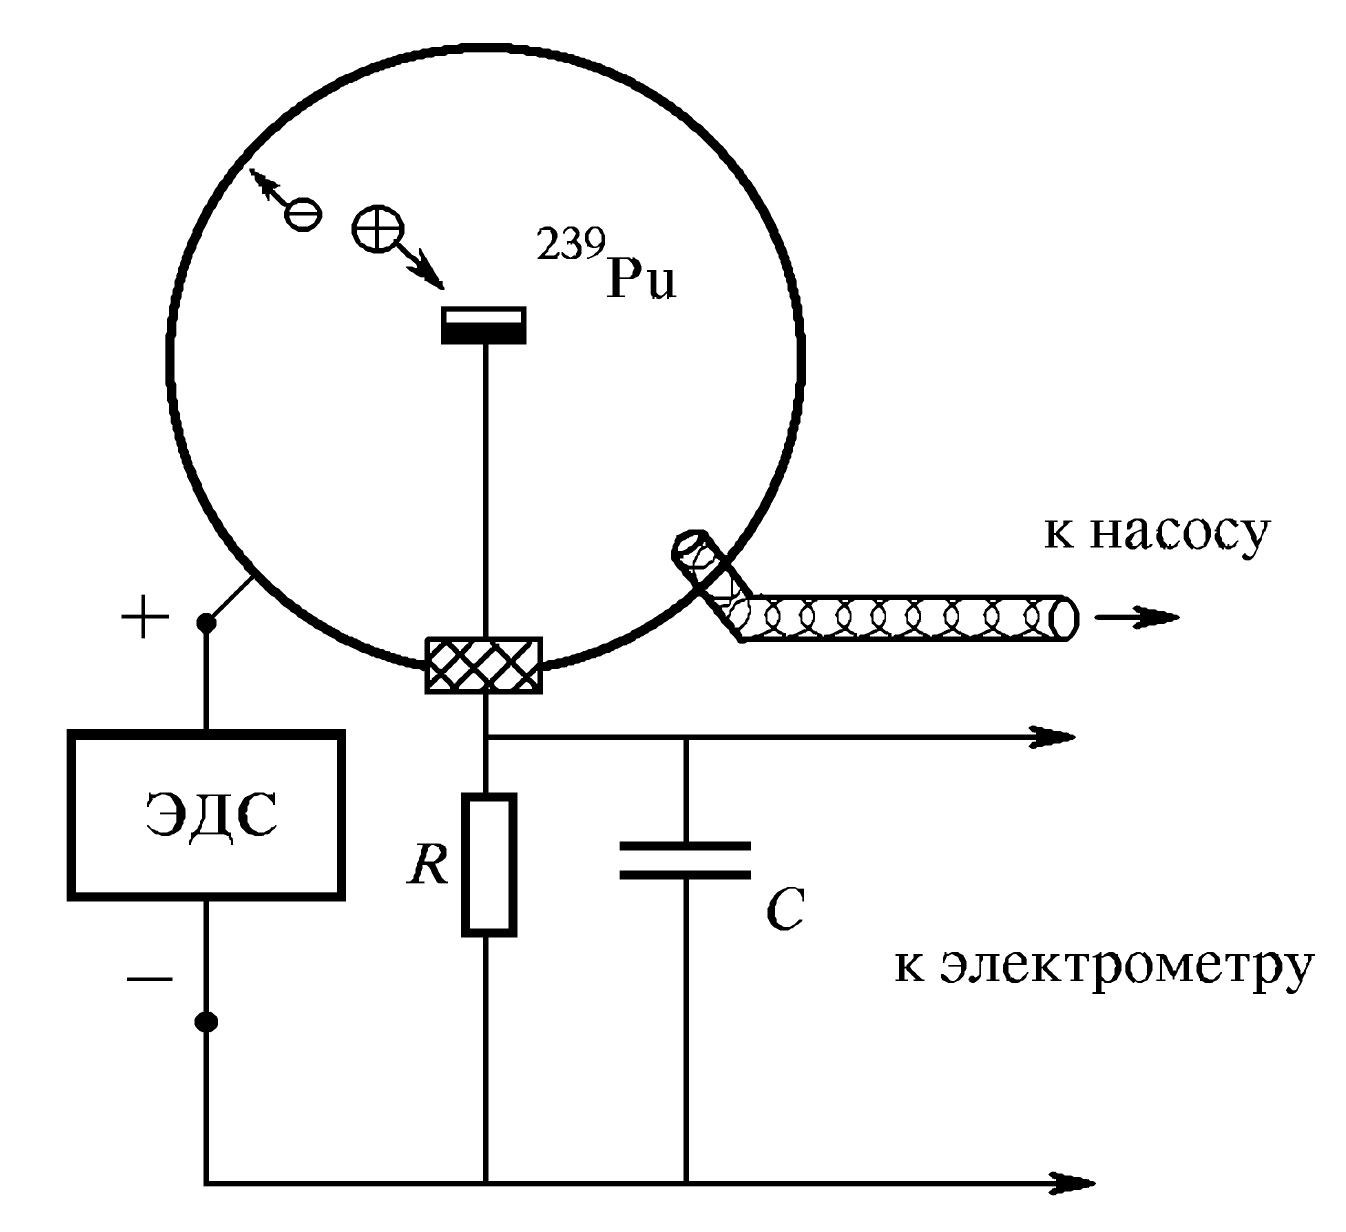
\includegraphics[scale=0.3]{Ion.png}
        \caption{Схема установки}
        \label{fig:Ion}
    \end{figure}
    
    Включив питание установки, измерим ток при атмосферном давлении. После этого откачаем воздух
    и снимем зависимость тока от давления в камере. Результаты измерений представим в таблице \ref{table:exp1}.

    \begin{table}[h!]
    \begin{tabular}{|c|c|c|c|}
    \hline
    $P_{\text{приьор}}$, мм. рт. ст. & $P$, мм. рт. ст. & $I$, pA & $I_1$, pA \\ \hline
    720                              & 18,8             & 9       & 0         \\ \hline
    710                              & 28,8             & 25      & 16        \\ \hline
    680                              & 58,8             & 70      & 61        \\ \hline
    660                              & 78,8             & 102     & 93        \\ \hline
    640                              & 98,8             & 132     & 123       \\ \hline
    620                              & 118,8            & 165     & 156       \\ \hline
    600                              & 138,8            & 202     & 193       \\ \hline
    570                              & 168,8            & 249     & 240       \\ \hline
    540                              & 198,8            & 300     & 291       \\ \hline
    510                              & 228,8            & 346     & 337       \\ \hline
    480                              & 258,8            & 404     & 395       \\ \hline
    470                              & 268,8            & 429     & 420       \\ \hline
    450                              & 288,8            & 456     & 447       \\ \hline
    430                              & 308,8            & 494     & 485       \\ \hline
    410                              & 328,8            & 534     & 525       \\ \hline
    390                              & 348,8            & 576     & 567       \\ \hline
    370                              & 368,8            & 611     & 602       \\ \hline
    350                              & 388,8            & 652     & 643       \\ \hline
    330                              & 408,8            & 695     & 686       \\ \hline
    310                              & 428,8            & 735     & 726       \\ \hline
    290                              & 448,8            & 780     & 771       \\ \hline
    260                              & 478,8            & 845     & 836       \\ \hline
    230                              & 508,8            & 900     & 891       \\ \hline
    200                              & 538,8            & 930     & 921       \\ \hline
    180                              & 558,8            & 940     & 931       \\ \hline
    160                              & 578,8            & 940     & 931       \\ \hline
    140                              & 598,8            & 935     & 926       \\ \hline
    120                              & 618,8            & 935     & 926       \\ \hline
    100                              & 638,8            & 930     & 921       \\ \hline
    80                               & 658,8            & 925     & 916       \\ \hline
    50                               & 688,8            & 915     & 906       \\ \hline
    30                               & 708,8            & 910     & 901       \\ \hline
    0                                & 738,8            & 905     & 896       \\ \hline
    \end{tabular}
    \centering
    \caption{}
    \label{table:exp1}
\end{table}

    По полученным эксперементальным данным построим график зависимости $I(P)$. По графику определим точку перелома.

    \begin{figure}
        \centering
        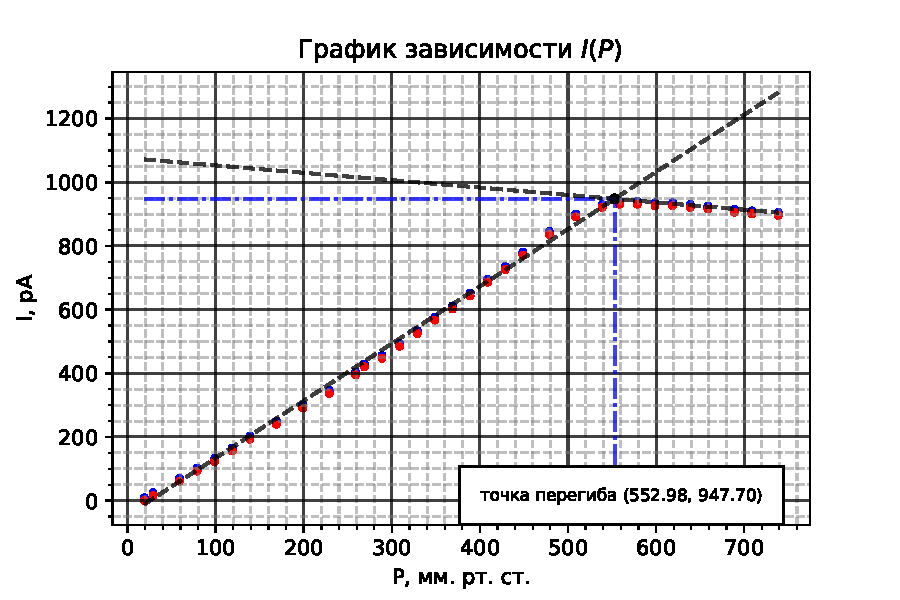
\includegraphics[width=\textwidth]{PI.pdf}
        \caption{}
        \label{fig:1}
    \end{figure}

    \begin{center}
        \fbox{$P_0 = 552.97$ мм. рт. ст.}
    \end{center}

    Приведем данный к нормальным условиям ($P_n = 760$ мм. рт. ст. $T_n = 15 ~ ^oC$), при условии,
    что пробег, задаваемый камерой $R = 5$ см.

    \[ R_n = R \frac{P_0 T_n}{P_n T_0} = 2.48 ~ \text{см} \]

    Выразим пробег в г/см$^3$:

    \[ R' = \rho R = 3.02 \cdot 10^{-3} ~ \text{г/см}^2 \]

    где $\rho$ -- плотность вещества (в нашем случае воздуха). $\rho(15 ~ ^oC) = 1.22 10^{-3}$ г/см$^2$.

    Используя формулу $R = 0.32 E^{\frac{3}{2}}$ оценим энергию $\alpha$-частицы.

    \[ E = \left(\frac{R}{0.32} \right)^{2/3} = 3.91 ~ \text{МэВ} \]

    Сравним полученные в ходе эксперемента величины с табличными значениями. Согласно табличным данным,
    Пробегу $\alpha$-частицы в воздухе $R = 2.37$ см соответствует энергия частицы $E = 4.0$. Отсюда
    можно сделать вывод, что полученный в ходе данного эксперемента значения достаточно хорошо соответствует 
    действительности.

    \section*{Сцинтилляционный счетчик}

    Используя установку снимим зависимость числа зарегистрированных за 10 с частиц от давления в установке.
    Результаты представим в таблице \ref{table:experement2}.

    \begin{table}[h!]
    \begin{tabular}{|c|c|c|}
    \hline
    $P_{\text{прибор}}$, мм. рт. ст. & $P$, мм. рт. ст. & $N$    \\ \hline
    720                              & 18,8             & 3602   \\ \hline
    660                              & 78,8             & 3439   \\ \hline
    640                              & 98,8             & 3276   \\ \hline
    630                              & 108,8            & 3073   \\ \hline
    620                              & 118,8            & 2893   \\ \hline
    610                              & 128,8            & 2743   \\ \hline
    600                              & 138,8            & 2534   \\ \hline
    590                              & 148,8            & 2344   \\ \hline
    580                              & 158,8            & 2181   \\ \hline
    570                              & 168,8            & 2034   \\ \hline
    560                              & 178,8            & 1761   \\ \hline
    550                              & 188,8            & 1656   \\ \hline
    540                              & 198,8            & 1370   \\ \hline
    530                              & 208,8            & 1124   \\ \hline
    520                              & 218,8            & 920    \\ \hline
    510                              & 228,8            & 737    \\ \hline
    500                              & 238,8            & 541    \\ \hline
    490                              & 248,8            & 370    \\ \hline
    480                              & 258,8            & 181    \\ \hline
    470                              & 268,8            & 170    \\ \hline
    460                              & 278,8            & 60     \\ \hline
    450                              & 288,8            & 10     \\ \hline
    420                              & 318,8            & 3      \\ \hline
    370                              & 368,8            & 2      \\ \hline
    330                              & 408,8            & 2      \\ \hline
    260                              & 478,8            & 2      \\ \hline
    130                              & 608,8            & 1      \\ \hline
    100                              & 638,8            & 1      \\ \hline
    \end{tabular}
    \centering
    \caption{}
    \label{table:experement2}
\end{table}

    По данным из таблицы \ref{table:experement2} построим график зависимости $N(P)$.

    \begin{figure}
        \centering
        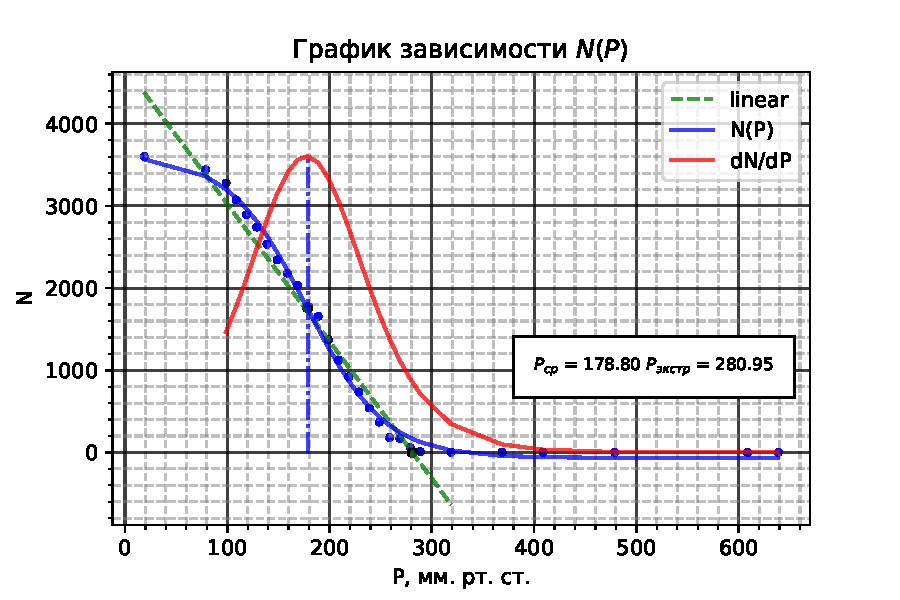
\includegraphics[width=\textwidth]{PN.pdf}
        \caption{}
        \label{fig:plot2}
    \end{figure}

    Экстрополируя линейную часть графика до пересечения с осью абцисс найдем величину $P_{extr}$, а так же
    $P_{\text{ср}}$, что соответсвует значениям $R_{extr}$ и $R_{\text{ср}}$.

    \begin{center}
        $P_{extr} = 280.95$ мм. рт. ст. $\Rightarrow$ $R_{extr} = 2.27$ см $\Rightarrow$ $E_{extr} = 3.69$\\
        $R_{\text{ср}} = 178.80$ мм. рт. ст. $\Rightarrow$ $R_{extr} = 1.44$ см $\Rightarrow$ $E_{\text{ср}}  = 2.72$
    \end{center}
\end{document}